
%......................................
\subsubsection{The Stenberg macro-element} 

This macro-element is introduced in \textcite{sten84} (1984). 

\input{tikz/tikz_stenberg}

Gresho \& Sani \cite{grsa} state: "For fans of $Q_1\times Q_0$ who want 
guaranteed optimal convergence of both $u$ and $p$ (with however larger error 
constants caused by the distorted shapes?), one way to assure this is
to discretise via the macro elements above, each composed of five $Q_1\times Q_0$
quadrilaterals. Such checkerboard-killer meshes have been employed in practice
by (at least) Bath\'e \cite{chba93}. Both the macro-element and the proof are
due to Stenberg \cite{sten84}."

Chapelle \& Bathe \cite{chba93}: "the numerical inf-sup test is passed for this mesh and in fact,
this behavior was proven analytically (see Brezzi \& Fortin \cite{brfo}, see 
also Le Tallec \& Ruas \cite{leru86}).

\begin{center}
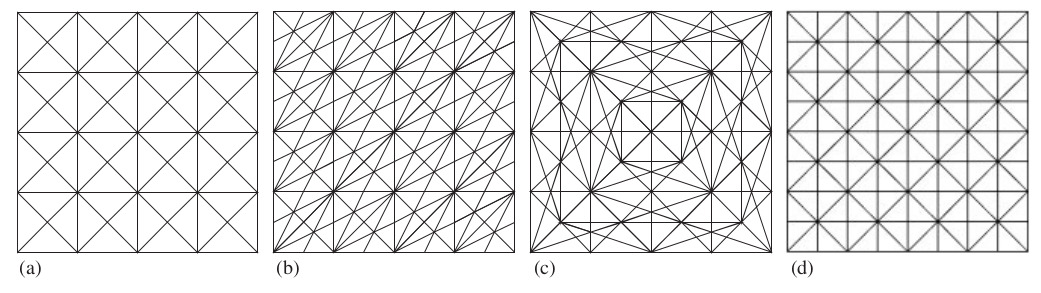
\includegraphics[width=5cm]{images/meshtopos/qizh07}\\
{\captionfont Taken from Qin \& Zhang (2007) \cite{qizh07}.}
\end{center}

Implemented in \stone~78.

\Literature: Fig 3.12 of Elman \etal book \cite{elsw}. Mentioned in \textcite{qizh07b} (2007).

%......................................
\subsubsection{The Le Tallec macro-element} 

This macro-element is introduced in \textcite{leta81} (1981).

\input{tikz/tikz_letallec}

This macro-element has been proven stable in \cite{leta81,leru86}, i.e. it satisfies 
the stability condition (see Section~\ref{ss:pair}).
It is also mentioned in Qin \& Zhang (2007) \cite{qizh07}.

Implemented in \stone 78.

%..............................................
\subsubsection{The Qin \& Zhang macro-elements}

In their paper \textcite{qizh07} (2007) the authors mention the Stenberg and Le Tallec
macro-elements and also introduce three new ones:

\begin{minipage}{0.31\textwidth}
\input{tikz/tikz_qizh07a}
\end{minipage}\hfill 
\begin{minipage}{0.31\textwidth}
\input{tikz/tikz_qizh07b}
\end{minipage}\hfill 
\begin{minipage}{0.31\textwidth}
\input{tikz/tikz_qizh07c}
\end{minipage}

They also indicate that although stable, these macro-elements are inferior 
to the above two (Stenberg \& Le Tallec). 

%..............................................
\subsubsection{New macro-elements ?}

\begin{center}
\includegraphics[width=4cm]{images/meshtopos/m21}
\includegraphics[width=4cm]{images/meshtopos/m22}
\end{center}

I came up with these, no idea whether these are stable/usable or better than the others.



